\documentclass[letter, 10pt]{article}
\usepackage[utf8]{inputenc}
\usepackage[spanish]{babel}
\usepackage{amsfonts}
\usepackage{amsmath}
\usepackage[pdftex]{graphicx}
\usepackage{epstopdf}
\usepackage{url}
\usepackage{hyperref}
\usepackage{verbatim}
\usepackage[top=3cm,bottom=3cm,left=3.5cm,right=3.5cm,footskip=1.5cm,headheight=1.5cm,headsep=.5cm,textheight=3cm]{geometry}


\begin{document}
\bibliographystyle{plain}
\pagestyle{empty}

\title{Inteligencia Artificial \\ \begin{Large}Informe Final: ``Car Sequencing Problem''\end{Large}}
\author{Cristián D. Maureira Fredes.}
\date{\today}
\maketitle


%--------------------No borrar esta sección--------------------------------%
\section*{Evaluación}

\begin{tabular}{ll}
Mejoras 1ra Entrega (10 \%): &  \underline{\hspace{2cm}}\\
Codigo Fuente (10 \%): &  \underline{\hspace{2cm}}\\
Representaci\'on (15 \%):  & \underline{\hspace{2cm}} \\
Descripci\'on del algoritmo (20 \%):  & \underline{\hspace{2cm}} \\
Experimentos (10 \%):  & \underline{\hspace{2cm}} \\
Resultados (10 \%):  & \underline{\hspace{2cm}} \\
Conclusiones (20 \%): &  \underline{\hspace{2cm}}\\
Bibliograf\'ia (5 \%): & \underline{\hspace{2cm}}\\
&  \\
\textbf{Nota Final (100)}:   & \underline{\hspace{2cm}}
\end{tabular}
%---------------------------------------------------------------------------%

\begin{abstract}
%Resumen del informe en no más de 10 líneas.
El presente documento tiene como finalidad presentar el estudio y análisis de un problema clásico, a lo que la Inteligencia Artificial respecta,
el \emph{Car Sequencing Problem}~\cite{parello}, que consiste en la planificación de una fila de vehículos en una línea de ensamblaje, 
mientras se satisfacen todas las restricciones de capacidad de las plantas ensambladores y de los propios vehículos.

La importancia de atacar el presente problema radica en el notorio aumento de la actividad en las fábricas automotrices a lo largo del mundo,
dejando como consecuencia que incluso para el pasado año 2002, ya existían 1 automóvil por cada 10 personas en el mundo~\cite{worldmapper}.

Se plantean además las técnicas más conocidas y utilizadas para poder enfrentar el presente problema, entre las cuales destacan la utilización
de heurísticas y métodos híbridos, dentro de los que son los acercamientos exactos, híbridos y mixtos.

Se presenta un modelamiento simplista utilizando lo que es Programación Lineal, y un planteamiento más teórico para poder comprender a fondo
el problema estudiado.



%problem
%solucion propuesta
%resultados
%keywords

\end{abstract}

\section{Introducción}
\label{sec:introduccion}
\frame
{
\frametitle{Introducción}
\begin{itemize}
	\item Motivación del problema.
	\item Sobre la técnica.
	\item Implementación inicial.
	\item Sintonización.
	\item \blue{Control}.
	\item Resultados.
\end{itemize}
}



\section{Definición del Problema}
\label{sec:definicion}
%Descripción del problema, su complejidad, en que consiste, cuales son sus objetivos,
%restricciones, variantes más conocidas. 

El \emph{Car Sequencing Problem} es un problema de satisfacción de restricciones (CSP), posee la
característica de ser NP-duro~\footnote{
NP-duro es el conjunto de los problemas de decisión que contiene los problemas H
tales que todo problema L en NP puede ser transformado polinomialmente en H.
Esta clase puede ser descrita como conteniendo los problemas de decisión que son
al menos tan difíciles como un problema de NP.}
, además corresponde a un tipo de variación del problema NP-completo \emph{Job-Shop Scheduling}.%,
%pero con un uso de razonamiento automatizado, es decir, con un enfoque dedicado a estudiar y comprender
%diferentes características del razonamiento, permitiendo así construir programas que le den la posibilidad
%a los computadores para razonar en forma autónoma.
 
Siguiendo la misma idea, es válido señalar que el \emph{Car Sequencing Problem} es un tipo de problema de planificación
de tareas en una línea de ensamblaje de autos, donde cada uno es perteneciente a un clase de automóvil, debido al conjunto
de opciones y accesorios que posee (airo acondicionado, centralizado eléctrico, etc), y cada una de las opciones o
accesorios se instala en una planta distinta, por lo que el objetivo principal es el poder encontrar el orden en la
secuencia de los vehículos, preocupándonos de no exceder la capacidad de cada planta de ensamblaje y también cumplir con la demanda.

Por lo tanto, si realizamos una definición más formal de nuestro problema, podríamos decir lo siguiente:
Teniendo una lista de vehículos dada, cada uno con sus respectivas opciones requeridas,
necesitamos establecer un orden en la línea de ensamblaje, con el fin de que cada subsecuencia de $q$ vehículos
tengamos a lo más $p$ que requieren de una determinada opción. Es importante tener en consideración que los
valores de $p$ y $q$ están asociados a cada opción de los vehículos.

Con respecto a la información que el problema otorga, podemos decir que contamos con:
\begin{itemize}
	\item Cantidad de vehículos de cada tipo o clase a producir (demanda)
	\item Lista de las opciones con la cual se constituye cada tipo o clase de vehículo, la cual puede utilizar una representación
		booleana para saber si cierto tipo de automóvil posee o no una determinada opción.
	\item Capacidad de las plantas que se preocupan de instalar la determinada opción.
\end{itemize}

Nuestro objetivo principal es:
\begin{itemize}
	\item Encontrar un orden en nuestra secuencia, que sirva para minimizar el costo por cada restricción insatisfecha.
\end{itemize}

Con respecto a las restricciones, tenemos que:
\begin{itemize}
	\item En cada subsecuencia de los $q$ vehículos, a lo más pueden haber $p$ que requieran de la opción determinada.
		Donde $p$ y $q$ son valores asociados a cada opción.
	\item La capacidad de cada planta de ensamblaje no puede ser excedida, es decir, cumplir con la demanda de cada automóvil
		sin abusar de una planta determinada.
	\item Por cada tipo de auto, el numero de autos de ese tipo debe ser secuenciado, es decir, todos los automóviles de cada clase
		deben estar presente en una secuencia determinada.
\end{itemize}





\section{Estado del Arte}
\label{sec:estado}
%Debe contener: técnicas usadas en su resolución (en general las que han sido mas
%efectivas a la fecha), mejores resultados, estrategias mas usadas en su resolución,
%representacion, movimientos, penalización, etc..


El \emph{Car Sequencing Problem}~\cite{parello} es presentado por primera vez en la \emph{Journal of Automated Reasoning},
del año 1986 en \emph{EEUU}, por \emph{B.D Parello}, \emph{W.C. Kabat} y \emph{L. Wos}, siendo una variación
del problema ya conocido en el área de la Inteligencia Artificial, como lo es el \emph{Job-Shop scheduling problem},
pero usando otro tipo de razonamiento, el \emph{Razonamiento automatiza}, de ésta manera logran enfocar su trabajo
en el problema que ocurre en las líneas de producción de automóviles.

Desde la publicación del presente problema hasta los últimos años, han aparecido en distintas conferencias a lo largo
del mundo, diferentes formas de atacar el problema, que nos llevan desde  ``programación lineal'', ``Evolutionary Approaches''
y ``Local search'' con sus variantes.

Las técnicas que han sido utilizadas hasta el momento, no han sido desarrolladas sólo por matemáticos, sino que por una amplia
gama de investigadores, que van desde científicos del área de la producción, física, biología y gestión.

No obstante, gracias a los avances que ha tenido el campo de la Inteligencia Artificial, han aparecido nuevas metodologías,
que se relacionan con otras áreas como lo son la computación evolutiva, genética,  redes neuronales, neurofisiología;
los cuales han realizado contribuciones importantes a los problemas que tienen que ver con la ``planificación'' (scheduling).
Lo anteriormente señalado afirma el hecho que los problemas relacionados con la ``planificación'' abarcan muchas áreas en el mundo,
y que los trabajos en dicha área no tienen que ver sólo con científicos computacionales.

A continuación se describen algunos de los métodos más importantes que han sido propuestos desde el año
en que el \emph{Car Sequencing Problem} fue dado a conocer en el mundo de la investigación científica.


\subsection{Acercamientos heurísticos}
Existen distintos acercamientos que se han propuesto, que tienen como objetivo principal
encontrar una solución óptima lo más rápido posible.
Los acercamientos descritos a continuación son \emph{búsqueda local (local search)},
\emph{greedy approach}, \emph{Ant colony Optimization} y por último, \emph{Algoritmos genéticos}

\subsubsection{Búsqueda Local (Local Search)}
La \emph{Búsqueda Local} puede ser utilizada en distintos problemas que se formulan
de una forma determinada para poder encontrar una solución que maximice un criterio alrededor de un número
de soluciones candidatas

Lo que hace la \emph{Búsqueda Local}, es moverse en su vecindario solución por solución en el espacio previamente establecido
de las soluciones candidatas, también conocido como espacio de búsqueda, hasta que una solución considerada \emph{óptima}
es encontrada ó se termina el plazo de tiempo para encontrar la solución, por otra parte, 
el vecindario va a estar definido netamente con respecto al modelamiento del problema.

Actualmente existen variadas aproximaciones propuestas sobre \emph{Búsqueda Local},
para resolver el presente problema.
La diferencia aquí, es que la mayoría de las propuestas son acercamientos más
genéricos, es decir, se han utilizado varios problemas para aplicar la propuesta
planteada y entre ellos se encuentra el problema en cuestión, como por ejemplo~\cite{DTWZ94}
que nos plantea una mejora en el sentido de una \emph{Estrategia de Búsqueda}, considerando
el conflicto mínimo con respecto a la heurística \emph{hill-climbing}~\footnote{
Técnica de optimización matemática, puede ser usada para resolver problemas con muchas soluciones.
Consiste en escoger una solución aleatoria (potencialmente no óptima) y comienza a
realizar pequeños cambios a dicha solución en cada iteración, en cada momento se va mejorando un poco más.
}
y ha propuesto un escape con respecto a los mínimos locales incrementando el peso de las
restricciones que no se cumplen.

Por otra parte existen otras propuestas que se han enfocado netamente en resolver éste problema,
como es el caso de ~\cite{PG02}, que considera los algoritmos de \emph{Búsqueda local}
que se basan en una representación de una permutación y la evaluación de las restricciones que no se
cumplen utilizando funciones de penalización.

De la misma forma tenemos el caso de lo que plantea Gottlieb et al. en \cite{GPS03}, quien se refiere
a una parte en especial de nuestro problema, la construcción de la secuencia inicial, por lo tanto
sabemos que en la mayoría de los casos, la secuencia inicial de vehículos, de donde parte la
\emph{Búsqueda Local}, es una permutación aleatoria de un conjunto de vehículos para comenzar
a ensamblarlos, sin embargo la propuesta nos señala el construir ésta secuencia inicial en una forma
\emph{Voraz (Greedy)}~\footnote{
se refiere a a realizar una elección del siguiente elemento considerando una función heurística de optimización,
con la esperanza de llegar a una solución general óptima.
}
, lo que queda claramente demostrado en dicha publicación,
debido a las grandes mejoras en el proceso de solución.

\subsubsection{Acercamiento Voraz (Greedy approaches)}
Teniendo en consideración el \emph{Car Sequencing Problem}, podemos construir una secuencia
en una forma \emph{Voraz (Greedy)}, eligiendo el siguiente vehículo de la secuencia
considerando una función heurística de optimización.
El primero acercamiento utilizando \emph{Greedy} fue propuesto por
Hindi and Ploszaski en 1994~\cite{HP94}. Volviendo al procedimiento anteriormente descrito, la idea
central que nos plantea Gottlieb et al. en \cite{GPS03}. Claramente, ahora la elección que podemos
realizar en cada paso de nuestro algoritmo, debe ser la más óptima, en otras palabras,
elegir el vehículo que posea el menor número de restricciones no satisfechas.

Matemáticamente hablando, podríamos decir lo siguiente:
Dado una secuencia parcial $\pi$, el siguiente vehículo es seleccionado entre los vehículos $c_j$
que minimice la siguiente función,
$$newViolations(\pi, c_j) = \sum_{o_{i}\in O}r(c_j,o_i)\cdot violation(lastCars(\pi\cdot <c_j>,q(o_i)),o_i)$$
donde $o_j$ es una opción del vehículo $c_j$ y donde $lastCars(\pi',k)$ es la secuencia compuesta de los
últimos $k$ vehículos de $\pi'$, si $|\pi'| \geq k$, en otro caso $lastCars(\pi' , k) = \pi')$.

El problema acá, es que por lo general, el conjunto de vehículos seleccionados que minimizan la función
$newViolations$, contiene más de un auto, por lo tanto acá viene otra decisión importante. ¿Cuál de esos
autos elegimos?, por lo que Gottlieb et al.~\cite{GPS03} nos señala que es necesario utilizar otra técnica heurística para 
romper dicha incertidumbre, de la misma forma propone 6 heurísticas distintas. La heurística que presente
un mejor desempeño es llamada \emph{``dynamic sum of utilization rates''}, la cual consta en que en cada paso
añadimos el vehículo que maximiza la suma de las tasas de uso de opciones necesarias, estas tasas de uso se actualizan
dinámicamente cada vez que añadimos un nuevo auto al final de la secuencia.

\subsubsection{Ant Colony Optimization (ACO)}
El algoritmo \emph{Ant Colony Optimization (ACO)}, tal como es descrito en \cite{DS05},
toma su inspiración en el comportamiento de ciertas especies de hormigas. La idea central
es notar que las hormigas depositan en el suelo una feromona, con el objetivo de marcar
un camino favorable para que los otros miembros de su colonia puedan seguirlo. Por lo tanto
\emph{ACO} busca aplicar un mecanismo similar para resolver problemas de optimización.

En otras palabras, \emph{ACO} es una forma de modelar cierto problema de tal forma
que busquemos siempre el camino con mínimo costo en un grafo determinado, y por supuesto,
utilizar \emph{hormigas artificiales} para buscar los caminos que más nos pueden favorecer.


El primer algoritmo de \emph{ACO} fue propuesto por Christine Solnon~\cite{Sol00},
y se trata de resolver un problema de satisfacción de restricciones de permutación~\footnote{
El objetivo principal es poder encontrar la permutación de $n$ valores conocidos,
para asignarlos a $n$ variables, bajo ciertas restricciones.
},
utilizando el concepto de \emph{hormigas artificiales}. Principalmente está diseñado
para resolver un problema general de combinatoria.

En enfoque que entrega el trabajo previamente señalado~\cite{Sol00} con respecto
al \emph{Car Sequencing Problem} es el siguiente:
Recordando nuestro problema principal, sabemos que consiste
en realizar la óptima planificación de los vehículos en una línea de ensamblaje,
donde tenemos $n$ vehículos para producir, que están agrupados en $k$ tipos
de autos~\footnote{
Cada conjunto de autos de un mismo tipo tienen las mismas opciones
}, y sabemos también que cada opción $i$ está asociada con una restricción de capacidad
representada por una tasa $p_i/q_i$, que especifica que para cualquier secuencia
de $q_i$ autos consecutivos en le línea de ensamblaje, tenemos al menos $p_i$ vehículos
que requieren dicha opción.
Finalmente el objetivo será encontrar una permutación de $n$ vehículos que satisfacen
todas las restricciones de capacidad, tomando en consideración que nuestra feromona
se pondrá sobre las parejas de los vehículos consecutivos con el fin de aprender
las sub-secuencias de vehículos más prometedoras (óptimas).

No conforme con el desempeño mostrado en el trabajo anterior, Gottlieb et al.~\cite{GPS03}
proponen un nuevo algoritmo que introduce tres nuevas mejoras:
\begin{itemize}
	\item Se utiliza una estrategia elitista, por lo que la feromona es usada para romper el lazo entre los mejores vehículos solamente.
	\item Se integran mejoras del trabajo ~\cite{Stu}, para favorecer la exploración.
	\item Se usan funciones heurísticas de tipo \emph{voraz (greedy)} para guiar las hormigas.
\end{itemize}
Con las mejoras anteriormente planteadas se logra obtener un resultado mucho más óptimo computacionalmente.

\subsubsection{Algoritmos Genéticos (Genetic Algorithms)}
Los \emph{Algoritmos Genéticos} son una técnica computacional que tienen como objetivo principal,
el encontrar una solución exacta o aproximada en problemas de optimización y búsqueda.

En el trabajo de Warwick y Tsang~\cite{WT95} se propone un algoritmo genético especialmente
para resolver el \emph{Car Sequencing Problem} que se diferencia de los algoritmos genéticos
tradicionales pues ingresa ciertas características especiales como el \emph{elitismo}~\footnote{
proceso de seleccionar mejores individuos, seleccionándolos con el fin de obtener una mejor solución
}, plantillas adaptativas de \emph{crossover}~\footnote{
operador genético utilizado para variar la programación de uno o varios cromosomas, de una generación  a otra.
}, \emph{hill-climbing}, entre otras.

El acercamiento que nos ofrece éste mecanismo tiene su origen en una especie de inspiración
de la evolución natural y trata de introducción computacionalmente los conceptos de \emph{cross over},
\emph{mutación}, y tomar las secuencias de nuestros problemas, como una \emph{población}.

Por lo tanto, el procedimiento que realiza es que por cada \emph{generación}, las secuencias
que son seleccionadas se combinan gracias al operador \emph{cross over}, y se obtiene lo
que se denomina \emph{descendencia} que puede que no satisfaga la restricción global,
pero se va reparando en cada iteración y luego se le aplica \emph{hill-climbing} mediante
una función de intercambio.

Lamentablemente el procedimiento anteriormente descrito es bueno para resolver sólo,
versiones no tan complejas del \emph{Car Sequencing Problem}.
Debido a lo anterior Cheng et al. \cite{CLP+99} propone un algoritmo para resolver un
problema práctico, es decir, más realista, con un grado mayor de complejidad.
Cheng et al. \cite{CLP+99} proponen un operador llamado \emph{cross-switching},
que genera una descendencia intercambiando los vehículos que aparecen de forma aleatoria
en la primera secuencia del problema.

\subsubsection{Movimientos}

A continuación se explican brevemente algunos movimientos conocidos que definen el vecindario de 
una solución, y que de la misma forma, es válido para cualquier acercamiento anteriormente
mencionado.
\begin{enumerate}
	\item \emph{shift}: Puede realizarse con repecto a la izquierda o derecha, y avanzando una cantidad determinada de espacios,
		es decir, tomamos nuestra secuencia numérica, y la movemos para alguno de los dos lados. El hecho de que sea a la izquierda
		o derecha y la cantidad de espacios que se mueve, se puede elegir de manera aleatoria.

		\emph{e.g:} 1 0 1 0 0 1, aplicamos shift-right 2 veces y nos queda 0 1 1 0 1 0.
	\item \emph{swap}: Este movimiento es muy utilizado, pues ha demostrado tener alta eficiencia al momento de buscar
		nuevas soluciones, sin romper restricciones. Consiste en tomar dos elementos de nuestra secuencia, que pueden ser escogido
		de forma aleatoria, e intercambiarlos
		de lugar.

		\emph{e.g:} 1 0 1 0 0 1, aplicamos swap(1,5) y nos queda 1 1 1 0 0 0.
	\item \emph{bit-flip}: Éste movimiento consiste en cambiar el valor de un \emph{bit} de nuestra secuencia numérica.
			Sólo es válida para representaciones binarias (0 o 1). Para escoger que elemento cambiamos, lo podemos hacer de una forma
			aleatoria.
		
		\emph{e.g:} 1 0 1 0 0 1, aplicamios bit-flip(3) y nos queda 1 0 1 1 0 1.
	\item \emph{Cruzamiento en un punto (Single Point Crossover)}: La presente técnica consiste en tener dos individuos,
		elegir un punto al azar dentro de la secuencia y cruzarlos, intercambiando su material. También existen otras variaciones
		de éste movimiento, donde se elige más de un punto para intercambiar el material de los padres.

		\emph{e.g:} 1 0 1 1 y 1 1 0 1, elegimos el punto 2 y nos quedan dos hijos de la forma, 1 0 0 1 y 1 1 1 1.
				
	\item \emph{Técnica incompleta}: Es posible utilizar una misma técnica incompleta como \emph{movimiento} para poder generar
		el vecindario determinado, lo cual en la mayoría de las veces, produce secuencias mucho mejor, pero toma mucho más tiempo
		que los movimientos descritos anteriormente.
\end{enumerate}

\subsection{Acercamientos completos}
\subsubsection{Integer Lineal Programming}
En el trabajo de Grevel et al.~\cite{4} se propone un acercamiento utilizando
\emph{Programación Lineal Entera}, ILP por sus siglas en inglés,  para una variante
del problema famoso de \emph{Car sequencing problem} pero del concurso ROADEF,
donde ahí se establece condiciones extras relacionadas a la pintura de los vehículos,
que éste modelamiento no posee.

Grevel et al.~\cite{4} también nos da a entender que se puede resolver el problema
de una manera común, con ésto nos referimos a usando un simple \emph{benchmark}
con aproximadamente unos $200$ vehículos y $5$ componentes, probando así
lo óptimo que es el método, con un tiempo de respuesta razonable.
La idea principal que posee éste mecanismo o modelamiento, es poder aplicarla a un
grupo de vehículos con la misma configuración, con respecto a las opciones,
evitando así simetrías entre ellos.

Existe otra aproximación relacionada con ILP, presentada por Prandtstetter et al.~\cite{12}
que es análoga a la formulación realizada por Gravel et al., clasificando los vehículos
que tienen la misma configuración en grupos, gracias a ésto el tamaño de alguna instancia
del problema que sea propuesto, está restringido a lo más $300$ vehículos con aproximadamente
unos $8$ componentes.

\subsubsection{Ramificación y Poda (Branch-and-bound method)}

El presente método es una variación del algoritmo \emph{Backtracking}~\footnote{
la idea del algoritmo se asemeja a un recorrido en profundidad dentro de un grafo dirigido.
}
, pero con bastantes mejoras.
Por lo general, la idea es interpretar el problema como un árbol de soluciones,
en el cual las ramas van a ser caminos para una posible solución, pero posterior a la solución
actual (rama actual).
La idea central del presente método es que se encarga de encontrar las ramas que no poseen
una solución óptima en comparación al resto y las \emph{poda} para no utilizar el tiempo
de búsqueda en alguna rama que no sirva.

En el trabajo de Drexl et al.~\cite{DKM06}, se propone utilizar la misma técnica anteriormente
descrita.

Primeramente es un poco complicado por imaginarse el problema atacado del punto de vista
del \emph{Branch-and-bound}, debido a que se toma como un problema de grafos, pero lo que
Drexl et al.~\cite{DKM06} establece es que el método está basado en un esquema de ramificación
\emph{(branching)} original, que utiliza el concepto de \emph{Car sequencing state}, 
refiriéndose así a que cada \emph{Car sequencing state} está asociado a cada nodo del árbol
que podemos construir para resolver el presente problema.

Para comenzar el \emph{branching}, es necesario construir una secuencia $\delta$
asignando cada periodo $t\in {1,...,V}$ a una copia de una variante $v$, realizando ésto
se puede manipular la secuencia $\delta$ de la forma:
$$\delta : \{1,...,T\}\rightarrow\{1,...,V\}\cup\{0\}$$~\footnote{
Se agrega el $0$ para evitar las secuencias parciales, asumiendo que ningún periodo no asignado
está siendo proyectada a una variante vacía. Ésto simplifica las definiciones, sin restringirlas.
}, con
\begin{itemize}
	\item $T:$ volumen total de producción (periodos, ciclos), i.e $T=\sum\limits_{v=1}^{V}D(v)$, índice $t$
	\item $V:$ número de variantes, índice $v$
\end{itemize}

La secuencia $\delta$ induce una matriz $O\times T$ que llamaremos $M$,
la cual está representando los periodos de la planificación de T,
y cada file de $M$ incide con una opción $j$
, con
\begin{itemize}
	\item $O:$ número de opciones, índice $j$.
\end{itemize}

La interpretación de la matriz de la matriz $M$ se define a continuación:\\

$m_{j,t} = \left\{ \begin{array}{l}
\ \ 1,\ \text{si la opción}\ j\ \text{es planificada en el periodo}\ t,\ \text{respetando la restricción}\ H_{j}:H_{j}\\
\ \ 0,\ \text{si la opción}\ j\ \text{puede ser planificada en el periodo}\ t\\
-1,\ \text{si la opción}\ j\ \text{no es planificada en el periodo}\ t\text{, si es planificada puede violar}\\
\ \ \ \ \ \text{la restricción}\ H_{j}:H_{j}\\
\end{array} \right.$

\subsubsection{Constraint Programming}

El método \emph{Constraint Programming} es una herramienta genérica para poder resolver problemas
del tipo \emph{Constraint  Satisfaction Problem (CSP)}~\footnote{No confundir con Car Sequencing Problem},
por lo tanto cualquier problema de \emph{scheduling} puede ser resuelto mediante ésta forma,
ya que conjunto de restricciones que debemos satisfacer son una relación entre varias variables desconocidas,
y otras variables conocidas~\cite{Tsa93}.

%
Por lo general para obtener una solución óptima, se suelen combinar técnicas heurísticas,
y otras para deducir restricciones derivadas, como la clausura.
Como es el caso de Alfonso y Barber~\cite{esp1}, el cual utiliza un método primero de \emph{constraint-posting},
que significa ir adicionando sucesivamente las restricciones y en cada paso realizar el proceso de clausura,
en otras palabras incorporan el proceso de clausura que determina el conjunto de las restricciones que pueden
impedir  en las que ya se han asertado correctamente.

Dejando de lado el trabajo anteriormente mencionado, el método de \emph{Constraing Programming} permite la definición
y aplicación de nuevas técnicas de heurística, permitiendo así limitar el número de disyunciones
del conjunto de las restricciones y además permiten dirigir mejor el proceso de búsqueda.

\subsection{Acercamientos híbridos}

Cuando hablamos de acercamiento híbrido, nos referimos a poder combinar las ventajas de varios
métodos de optimización en un sólo algoritmo.
Anteriormente vimos que en muchos casos, existe inclusive una \emph{recomendación} para buscar
una heurística determinada complementando a un método y encontrar una solución óptima.


Tomando las palabras del estudio realizado por E.G Talbi~\cite{talbi} los algoritmos híbridos
se han aplicado satisfactoriamente a variados problemas de optimización combinatorial, como el problema
del \emph{vendedor-viajero} o simplemente problemas del mundo real.


Siguiendo las palabras de Blum, Roli y Alba en ~\cite{blum} podemos aseverar que ésta clase de acercamientos,
combinando metaheurísticas basadas en  poblaciones con alguna solución metaheurística simple, podemos llegar
a la conclusión de que es el mejor camino para poder mejorar la calidad de las soluciones que encontramos
en cualquier problema de optimización.

\subsubsection{Hybrid Integrative Evolutionary Approaches}
En el trabajo de Zinflou et al. \cite{HYB1} se presentan tres acercamientos para poder
resolver el presente problema. Los acercamientos están basados en esencia en algoritmos evolutivos
que incorporan operadores de heurística como los son los \emph{crossover operators} usando
un modelo simple, es decir basado en  Programación Lineal Entera.

La diferencia que existe entre dos de las aplicaciones de \emph{crossover} combinadas nos muestra que es posible
obtener valores competitivos, dignos de ofrecer como alternativa a los métodos anteriormente nombrado, debido
a la calidad de la solución.

Finalmente podemos darnos cuenta que la experiencia numérica de la formulación de éste método, muestra una diferencia
notoria en el tiempo de ejecución, algoritmicamente hablando.
Las diferencias indican que puede ser posible de obtener mejoras en la implementación de métodos híbridos para 
poder obtener una comparación más competitiva. Dichas mejoras significan poder involucrar al desarrollo de nuestro
algoritmos un enfoque de \emph{Grid computing} u otras técnicas de \emph{high performance computing technologies}.


\section{Modelo Matemático}
\label{sec:modelo}
%Uno o más modelos matemáticos para el problema, idealmente indicando el espacio de búsqueda para cada uno.
\subsection{Primer modelo}
El presente modelo, pese a utilizar notaciones matemáticas, trata de dar un enfoque más teórico,
para una mejor comprensión del problema.

Consideremos el \emph{Car Sequencing Problem} como una tupla $(C,O,p,q,r)$, tal que:
\begin{itemize}
	\item $C=\{c_1,\ldots,c_n\}$ es el conjunto de vehículos a producir.
	\item $O=\{o_1,\ldots,o_m\}$ es el conjunto de distintas opciones.
	\item $p:O\rightarrow\mathbb{N}$ and $q:O\rightarrow\mathbb{N}$ definen la capacidad de las restricciones,
		es decir, para cualquier opción $o_i \in O$, cada subsecuencia de $q_i$ vehículos consecutivos en la línea,
		deben no contener más que $p_i$ vehículos que requieran la opción $o_i$
	\item $r:C\times O \rightarrow \{0,1\}$ define los requerimientos de las opciones, es decir, para cada vehículo
		$c_i \in C$ y para cada opción $o_j \in O$, $r_{ij} = 1$ si $o_j$ debe ser instalado en $c_i$ y $r_{ij} = 0$
		en otro caso.
\end{itemize}

%Solving a car sequencing problem involves finding an arrangement of the cars
%in a sequence, defining the order in which they will pass along the assembly
%line, such that the capacity constraints are met. We shall use the following
%notations to denote and manipulate sequences:

\begin{itemize}
	\item Una \emph{secuencia}, definida $\pi =< c_{i_{1}}, c_{i_{2}}, \ldots, c_{i_{k}} >$, es una sucesión de vehículos.
	\item El conjunto de todas las secuencias que pueden ser construidas con un conjuntos de autos $C$ es denominada $\amalg_{C}$.
	\item El \emph{largo} de una secuencia $\pi$, denominado $|\pi|$, es el numero de vehículos que contiene.
	\item La \emph{concatenación} de dos secuencias, $\pi_1$ y $\pi_2$, denominada $\pi_1 \cdot \pi_2$, es una secuencia
		compuesta de los vehículos de $\pi_1$ seguidos de los vehículos de $\pi_2$.
	\item Una secuencia $\pi_1$ es una subsecuencia de otra secuencia $\pi_2$ , tomando en cuenta $\pi_1 \subseteq \pi_2$,
		si existen dos secuencias $\pi_3$ y $\pi_4$, tal que $\pi_2 = \pi_3 \cdot \pi_1 \cdot \pi_4$
	\item El \emph{cost} de una secuencia $\pi$ es el numero de las restricciones de capacidad que no se cumplen, es decir:
\end{itemize}

$$costo(\pi) = \sum_{o_{i}\in O} \ \ \ \sum_{\pi_{k}\subseteq \pi\\ \rightarrow |\pi_{k}|=q_i} violaci\acute{o}n(\pi_{k},o_{i})$$
$$\text{donde}\ violaci\acute{o}n(\pi_{k},o_{i}) = \left\{
 \begin{array}{l}
	0\ si\ \sum\limits_{<C_l>\subseteq\pi_k}r_{li}\leq p_i;\\
	1\ \text{en otro caso}\\
 \end{array} \right.$$


Por lo tanto se puede resolver ahora el ejercicio buscando la secuencia con el \textbf{mínimo costo}, compuesta por todos los autos
que serán producidos.

%

Respecto al espacio de búsqueda, si tenemos que $\alpha_o$ es la cantidad de vehículos que tienen que ser producidos
por cada clase/configuración o, con $o\in O$ y sea $n$ la cantidad total de vehículos a producir,
entonces el espacio de búsqueda está compuesto por todas las posibles permutaciones de los vehículos en $C$ que
requieren diferentes configuraciones, particionado en los $o$ tipos distintos tipos de vehículos a construir.

Por lo tanto el tamaño de las posibles soluciones sería:
$$E.B\ =\ \frac{n!}{\prod\limits_{o \in O}\alpha_o}$$
 
Claramente tenemos que darnos cuenta que varias soluciones dentro del presente espacio de búsqueda
no van a ser posibles, pues debemos aplicar las restricciones.

\subsection{Segundo modelo}
\textbf{Programación Lineal Entera (ILP)}

Definición de \emph{variables} y \emph{parámetros}:
\begin{itemize}
	\item \textbf{$opt$}	    Número total de opciones.
	\item \textbf{$cl$}	    Número total de tipos/clases de vehículos.
	\item \textbf{$n_i$}    Número de vehículos en la clase/tipo $i$.
	\item \textbf{$nc$}	    Número total de vehículos.
	\item \textbf{$o_{ik}$}	Parámetro \emph{booleano} que representa si los vehículos del tipo/clase $i$ requieren la opción $k$.
	\item \textbf{$s_k$}    Largo de una secuencia de vehículos consecutiva, donde algunas requieren la opción $k$
	\item \textbf{$r_k$}    Número máximo de vehículos que pueden tener la opción $k$ en una secuencia consecutiva de $s_k$ vehículos.
	\item \textbf{$M$}	 	Valor escalar grande que puede ser fijado a $(s_{k} - r_{k})$
	\item \textbf{$C_{ij}$}	Variable \emph{booleana} que representa si un vehículo del tipo/clase $i$ es asignado a la posición $j$ en la secuencia
		$(C_{ij} = 1)$
	\item \textbf{$Y_{kj}$}	Varibale \emph{booleana} que representa si el número de vehículos que requieren la opción $k$ en una secuencia
		de $s_k$ vehículos, comenzando de la posición $j$ en la secuencia respecto a $r_k$, el máximo permitido $(Y_{kj} = 0)$
	\item \textbf{$pp$}	    Número de vehículos en el periodo anterior, que permiten establecer la transición $(pp = max(s_{k}-1))$
	\item \textbf{$cpp_{mk}$}	Variable \emph{booleana} que representa si el vehículo $m$-ésimo del periodo previo tiene la opción $k$.
	\item \textbf{$Z_{kj}$}	Variable \emph{booleana} que representa si el número de vehículos que necesitan la opción $k$ en una secuencia
		de $s_k$ vehículos, partiendo en la posición $j$ de la secuencia en el periodo anterior, respetando el máximo $r_k$ permitido $(Z_{kj} = 0)$.
\end{itemize}

Por lo tanto, el modelo a continuación se establece para minimizar el número de violaciones de las restricciones de capacidad,
tanto como para opciones de alta prioridad, como de baja.

\textbf{Función objetivo:}
$$\text{Min} F = \sum\limits_{k=1}^{opt} \sum\limits_{j=1}^{nc-s_{k}+1} Y_{kj} + \sum\limits_{k=1}^{opt} \sum\limits_{j=1}^{s_{k}-11} Z_{kj}$$

\textbf{Restricciones}
\begin{itemize}
	\item Una sola clase de autos se puede asignar a cada una de las posiciones de la secuencia:\\ 
		$\sum\limits_{i=1}^{cl} C_{ij} = 1$, $\forall j = 1,\ldots,nc$
	\item Todos los autos de todas las clases serán incluidos en la secuencia:\\
		$\sum\limits_{j=1}^{nc} C_{ij} = n_{i}$, $\forall i = 1,\ldots,cl$
	\item Restricción de proporción, del tipo $r_{k}/s_{k}$ relacionada con las opciones del periodo actual, mientra que al mismo tiempo que se permite
		que sean violadas si las hya, de lo contrario no hay soluciones factibles:\\
		$\sum\limits_{i=1}^{cl} \sum\limits_{l=j}^{j+s_{k}-1} o_{ik} \cdot
		C_{il} \leq r_{k} + M\cdot Y_{kj}$, $\forall k = 1,\ldots,opt$ y $\forall j=1,\ldots, nc-s_{k}+1$
	\item Restricción de proporción, similar a la anterior, pero esta vez considera la transición entre un estado anterior y uno actual:\\
		$\sum\limits_{i=1}^{cl} \sum\limits_{l=1}^{j} o_{ik} \cdot
		C_{il} + \sum\limits_{m=pp-S_{k}+j+1}^{pp} cpp_{mk} \leq r_{k} + M\cdot Z_{kj}$, $\forall k = 1,\ldots,opt$ y $\forall j=1,\ldots, s_{k}-11$
\end{itemize}

Respecto al espacio de búsqueda, como ésta formulación es ILP igual que el primero modelamiento, sólo sería la permutación de todos
los vehículos que se necesitan,  particionados por las clases de vehículos que se producirán. Obviamente posicionándonos en el peor de los casos
donde tenemos que recorrer todo el espacio de búsqueda.

$$E.B\ =\ \frac{nc!}{\prod\limits_{i = 0}^{cl}\alpha_{n_i}}$$

Por ejemplo, si tuviéramos $30$ vehículos a ensamblar, $4$ clases de autos y
necesitamos $10$ autos de clase $1$, $5$ de clase $2$, $7$ de clase $3$ y $8$ de clase 4.

$$E.B\ =\ \frac{30!}{10\cdot 5\cdot 7\cdot 8}\ =\ 9.473316\times 10^{28}$$

%In the objective function we have used the “sliding window” method for counting the number of constraint violations, be they HPO or LPO, that is found in much of the existing literature [2], [12], [18]  B.D. Parello, CAR WARS: The (almost) birth of an expert system, AI Expert 3 (1988), pp. 60–64.[18] and [19]. Note that this method tends to amplify the number of option constraint violations by double counting. Consider, for example, an option that should be present in only one car in three in the sequence. By the current method of evaluation, the sequence (1 0 1 1 0 0) is said to have three violations in the windows (1 0 1), (0 1 1) and (1 1 0). In fact, the same two cars cause the latter two conflicts and removing either one or the other of them from this part of the sequence will solve both conflicts. In reality, the assembly line will be overloaded only twice and not three times as the evaluation method seems to indicate. Nevertheless, the “sliding window” method is used in the SA algorithm of Groupe Renault, and not without reason. The objective function is not so much intended to count the number of violations but rather to serve as a weighting function that forces the algorithm to disperse ‘problem vehicles’ throughout the sequence, thus reducing the total number of violations and easing production management in the plant. We have retained this form of objective function in our numerical experiments because this allows us to compare our results to those previously found via the SA algorithm of Groupe Renault. In our conclusions, we propose a new form of the capacity constraints that will avoid double counting in the objective function.
%
%The solution of the ILP of Model 1 will take the form of a car sequence that will minimize the number of capacity constraint violations linked to high-priority or low-priority options in the assembly shop. Given that the color of each vehicle has, as yet, not been considered in the model it is possible that this solution will not, in reality, be feasible in the plant. When a color is assigned to each vehicle of such a sequence, it may prove impossible to respect the maximum limit on consecutive vehicles of the same color in the paint shop. To include this factor in the model, we propose to include the car color in the definition of the decision variable and to add constraints on the maximum length of a sub-sequence of cars of the same color.


%%%

\section{Representación}
\label{sec:representacion}
% Descripción detallada de la representación elegida.

A continuación se explica la representación del algoritmo implementado,
que consiste en un \emph{Algoritmo Inmune} utilizando \emph{Selección Clonal}.

\subsection{Representación Matemática}

La presente representación, tiene un carácter simplista, y toma la esencia del modelo
matemático señalado en la sección anterior, buscando en éste caso, dar prioridad a la satisfacción
de la restricciones del problema, de una forma más apropiada.

\begin{itemize}
	\item Parámetros
	\begin{itemize}
		\item $cN$: Número total de autos.
		\item $oN$: Número total de opciones disponibles.
		\item $tN$: Número total de tipos/clases de autos.
	\end{itemize}
	\item Variables
	\begin{itemize}
		\item $nMax_{ij}$: Número máximo de autos con la opción $i$ en una subsecuencia $j$.
		\item $n_{ij}$: Número de autos con la opción $i$ en una subsecuencia $j$.
		\item $sMax_{i}$: Tamaño de la subsecuencia $j$ donde deben haber $nMax_{ij}$ autos.
		\item $q_{k}$: Cantidad de autos del tipo/clase $k$.
		\item $types_{il}$: Booleano que indica si la opción $i$ está presente en el auto $l$.
	\end{itemize}
	\item Función Objetivo
	$$FO\ :\ Min\ \sum\limits_{i=1}^{oN} \sum\limits_{l=1}^{cN} \sum\limits_{j=0}^{sMax_{i}} types_{il}\cdot (n_{ij} - nMax_{ij}), \forall n_{ij} > nM_{ij}$$
	\item Restricciones Duras
	$$\sum\limits_{k=1}^{cN} q_{k} = cN$$
	\item Restricciones Blandas
	$$\sum\limits_{i=1}^{oN} \sum\limits_{l=1}^{cN} \sum\limits_{j=0}^{sMax_{i}} types_{il}\cdot n_{ij} \leq nMax_{ij}$$
\end{itemize}
\subsection{Representación en Estructuras de datos}
La presente representación, posee una alta similitud con la representación matemática, buscando así presentar un código simple
con respecto a la satisfacción de restricciones y función objetivo.

\begin{itemize}
	\item Individuos ($\textbf{struct}\ cell$):
				
		Cada célula de nuestra población, corresponde a una secuencia de autos, más algunos atributos del mismo, por lo tanto,
		para representarlo es necesaria una estructura que posee los siguientes atributos:
		\begin{itemize}
			\item $\textbf{int}\ gene[VARS]$: Arreglo de enteros que corresponden  a la secuencia de autos, en su respectivo orden.
			\item $\textbf{int}\ fitness$: Corresponde a la aptitud de cada individuo, la cual tiene un valor correspondiente a las unidades
				extra por cada opción que sobrepase al máximo de autos permitidos con una cierta opción en una determinada subsecuencia.
			\item $\textbf{double}\ rfitness$: Corresponde a la aptitud relativa de cada individuo, la cual tiene un valor correspondiente
				a una probabilidad relacionada con su \emph{fitness}, la cual será explicada más adelante cuando se hable de la \emph{Selección de
				individuos}.
			\item $\textbf{double}\ cfitness$: Corresponde a la aptitud acumulativa de cada individuo, la cual tiene un valor correspondiente
				a una secuencia de probabilidades relacionadas con su \emph{fitness}, la cual será explicada más adelante cuando se hable de la \emph{Selección
				de individuos}.
		\end{itemize}

	\item Número máximo de autos por subsecuencia ($\textbf{int}\ numMaxCarOptSeq[N]$):
	
		Corresponde a un arreglo de enteros, que representa el número máximo de autos con la opción determinada, en una subsecuencia se nuestro individuo.


	\item Tamaño subsecuencia ($\textbf{int}\ sizeMaxCarOptSeq[N]$):

		Corresponde a un arreglo de enteros, que representa el tamaño de la subsecuencia donde debe haber un número máximo de opciones en un auto (numMaxCarOptSeq).

	\item Demandas y descripción de los tipos de autos ($\textbf{int}\ types[N][M]$):
	
	Corresponde a un arreglo bidimensional, que posee la siguiente información:
	\begin{itemize}
		\item $[N]$ posee sólo el valor del índice de la cantidad de tipos/clases de autos.
		\item $[M]$ posee el valor del índice anterior para cada tipo/clase , demanda del tipo de auto, y para cada opción si la posee o no (1 o 0).
	\end{itemize}
	\item Constantes:

		\begin{itemize}
			\item \emph{VARS(200, 300, 400)}: Número de autos.
			\item \emph{POP (160)}: Tamaño población
			\item \emph{GENS (2000)}: Número máximo de generaciones.
			\item \emph{N (128)}: Variable para crear arreglos determinados.
			\item \emph{clonationRate (POP*0.8)}: Tasa para realizar la clonación.
			\item \emph{replaceRate (POP*0.5)}: Tasa para la cantidad de elementos reemplazados.
			\item \emph{clonationFactor (0.8)}: Factor para calcular individuos clonados.
		\end{itemize}

\end{itemize}


\section{Descripción del algoritmo}
\label{sec:descripcionAlgoritmo}
% Como fue implementando, interesa la implementaci\'on m\'as que el algoritmo gen\'erico,
%  es decir, si se tiene que implementar SA, lo que se espera es que se explique en pseudo
%  codigo la estructura general y en parrafo explicativo cada parte como fue implementada
%  para su caso particular, si se utilizan oparadores se debe explicar por que se utilizo

%  ese operador, si fuera el caso de una t\'ecnica completa, si se utiliza recursi\'on o no,
%  etc. En este punto no se espera que se incluya codigo, eso va aparte.
El algoritmo utilizado para resolver el \emph{Car Sequencing Problem (CSP)} fue un
\emph{Algoritmo Evolutivo} con mutación \emph{Simulated Annealing}.

Las siguientes sub-secciones describen con más detalle como se adaptó la teoría de
los presentes algoritmos para resolver el \emph{CSP}.

\subsection{Población Inicial}
Una de las cosas mas importantes a la hora de evaluar si una solución es viable o no,
es su factibilidad, es decir, si cumple con todas las \emph{restricciones duras}.

Para solucionar lo anterior es que al momento de crear \emph{la población inicial},
se realizó de una forma aleatoria, pero cumpliendo con todas las \emph{restricciones
duras}, es decir, generando sólo \emph{restricciones factibles}.

Primero que todo se generó una secuencia ordenada con la cantidad de tipos de autos
requerida, es decir, si tuviéramos las siguientes demandas:
\begin{itemize}
	\item Tipo 1: 2 autos.
	\item Tipo 2: 1 auto.
	\item Tipo 3: 3 autos.
	\item Tipo 4: 6 autos.
\end{itemize}
La secuencia generada sería:

$$1\ 1\ 2\ 3\ 3\ 3\ 4\ 4\ 4\ 4\ 4\ 4$$

Una vez tengamos la secuencia, procedemos a generar todos los individuos de nuestra población
inicial, lo cual se realizó, desordenando la secuencia anterior, de una forma aleatoria.

% conclusión
Si nos damos cuenta, la forma de generar nuestra población, quizás no es la más adecuada
debido a que se generó de manera aleatoria, pero al generar solo soluciones factibles,
estamos mejorando mucho más éste aspecto, sin embargo, la utilización de  una técnica para
la construcción de soluciones iniciales, podría mejorar el performance de nuestro algoritmo,
por ejemplo si utilizáramos una técnica \emph{Greedy} o \emph{GRASP}.

\subsection{Evaluación de la población}

Para realizar la evaluación de una determinada población, se tiene en cuenta lo siguiente:

Es necesario recorrer toda la población, luego, una vez seleccionado un individuo, se procede
a recorrer mediante subsecuencias (de tamaño establecido en el problema, $sizeMaxOptCarSeq$)
todo el individuo (serie de autos), y por cada iteración vamos verificando si se cumplen las
restricciones blandas, es decir, sumamos la cantidad de autos con una opción determinada y
luego verificamos si esa suma es menor o igual al máximo permitido por las restricciones ($numMaxOptCarSeq$).

Si por cada suma en cada subsecuencia, no se cumple la restricción, se le asigna un \emph{fitness}
equivalente a las unidades por las cuales se excede el máximo establecido, al individuo en cuestión.

Finalmente, si encontramos alguna restricción factible que posea un \emph{fitness} igual a $0$,
inmediatamente, nos quedamos con dicha solución y el algoritmo termina.

\subsection{Selección de Individuos}

Al momento de seleccionar un individuo para realizar una transformación, se utilizó la conocida técnica llamada
\emph{roulette wheel}, para una Función Objetivo que minimiza.

El procedimiento es bien simple, sólo tenemos que considerar el \emph{fitness} de cada individuo y calcular un
\emph{fitness relativo} de la siguiente forma:

$$relativeFitness_{i}\ = \frac{f_{min} + f_{max} - f_{i}}{\sum\limits_{i=0}^{sizePop} (f_{min} + f_{max} - f_{i}}$$

Donde $f_{max}$ equivale al \emph{fitness} del mejor individuo,
$f_{min}$ equivale al \emph{fitness} del peor individuo y 
$f_{i}$ equivale al \emph{fitness} del i-ésimo individuo de nuestra población.

La suma de todos los \emph{fitness relativo} equivale a $1$.

Luego de que cada individuo posee su \emph{fitness relativo}, se procede a calcular un \emph{fitness acumulativo},
es decir, ir sumando las probabilidades para generar un rango entre $0$ y $1$ con todas nuestras probabilidades.

Una vez se tiene el \emph{fitness acumulativo} listo, se procede a obtener un número aleatorio entre $0$ y $1$,
para que luego sea ubicado en nuestro rango, y así el individuo que salga escogido con éste número aleatorio, será
elegido para pasar ahora a la transformación.

El siguiente ejemplo, ayuda a la comprensión del presente procedimiento:\\

\begin{minipage}{0.2\textwidth}
	\begin{tabular}{|r|r|}
	\hline
	\textbf{individuo} & \textbf{Fitness} \\ \hline
	1 & 50 \\\hline
	2 & 30 \\\hline
	3 & 20 \\\hline
	\end{tabular}
\end{minipage}
\  \ 
\hfill \begin{minipage}{0.2\linewidth}
	Tenemos ahora:
	\begin{itemize}
		\item $f_{min}$: 20
		\item $f_{max}$: 50
	\end{itemize}
\end{minipage}
\  \
\hfill \begin{minipage}{0.35\textwidth}
	\vspace{0.4cm}
	\begin{itemize}
		\item $f_{min}\ +\ f_{max}$: 70
		\item $\sum\limits_{i=1}^{3} (f_{min} + f_{max} - f_{i})$: 110
	\end{itemize}
\end{minipage}\\


Ahora procedemos a calcular el fitness relativo y acumulativo:\\

\begin{center}
\begin{tabular}{|r|r|r|r|}
\hline
\textbf{individuo} & \textbf{Fitness} & \textbf{Fitness relativo} & \textbf{Fitness acumulativo}\\ \hline
1 & 50 & 0.18 & 0.18 \\\hline
2 & 30 & 0.36 & 0.54 \\\hline
3 & 20 & 0.46 & 1.00 \\\hline
\end{tabular}
\end{center}

\begin{figure}[htb!]
	\begin{center}
	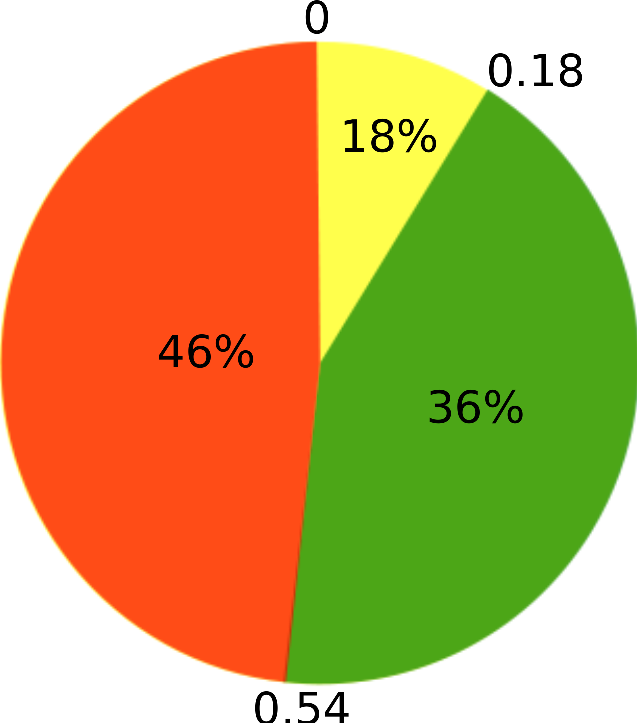
\includegraphics[scale=0.4]{img/fig1}
	\end{center}
	\label{fig:fig1}
	\caption{Gr\'afico final mediante el método de la ruleta}
\end{figure}

Si ahora escogiéramos un número aleatorio entre $0$ y $1$, por ejemplo $0.6$, tenemos que mirar la \textbf{Figura 1} de la sección~\ref{fig:fig1} y caeríamos
en el lugar del individuo 3, por lo que él sería escogido.

De esta forma, se les da una probabilidad a cada individuo para poder pasar a la nueva población, dependiendo
netamente de que tan bueno sea.

Este proceso se repite hasta que tenemos a todos los individuos de nuestra población nueva.


\subsection{Transformación de Individuos}

Por lo general, en las implementaciones de transformación, existe tanto la \emph{mutación} como el \emph{cruzamiento},
de los cuales, ambos poseen una cierta probabilidad asociada, para que cuando se escoja un individuo, se obtiene
un número aleatorio entre $0$ y $1$ y si ese número es menor o igual que la probabilidad de mutación, se muta,
lo mismo ocurre con el cruzamiento.

\subsubsection{Mutación}
Según los requerimientos del problema, la mutación debe ser la técnica \emph{Simulated Annealing} y se escogió la variación
de \emph{Alguna Mejora}, para obtener un menor tiempo de ejecución.

Pasos de la implementación:

\begin{itemize}
	\item Paso 0: Inicialización.
	\begin{itemize}
		\item X := solución inicial factible
		\item tmax := máximo número de iteraciones (IMAX)
		\item q := temperatura alta inicial (TMAX)
		\item Mejor solución := X
		\item Número de iteraciones = t := 0
	\end{itemize}
	\item Paso 1: Parada.
	\begin{itemize}
		\item Si la cantidad de iteraciones mayor a tmax o si la temperatura es menor que $0$,
			entonces paramos.
		\item Entregar mejor solución.
	\end{itemize}
	\item Paso 2: Movimiento.
	\begin{itemize}
		\item Realizamos el movimiento, en éste caso se realiza un \emph{swap},
			pero como cada individuo es del orden de $200$, $300$ y $400$ autos,
			se realiza una cantidad de \emph{swap} equivalente al $10\%$ de la cantidad de autos.
			
			Para ver que elementos hacen el \emph{swap}, se eligen aleatoriamente dos elementos para intercambiar.
		\item Calculamos la disminución de la FO (Dobj).
	\end{itemize}
	\item Paso 3: Aceptación.
	\begin{itemize}
		\item Si X(t+1) mejor el objetivo ó
		\item Si $e^{\frac{-Dobj}{q}}\ \ge\ random(0,1)$ entonces
		\item X(t+1) := X(t), sino
		\item volver al Paso 2.
		
	\end{itemize}
	\item Paso 4: Reemplazar el mejor.
	\begin{itemize}
		\item Si el valor de la FO de X(t+1) es mejor a la Mejor Solución, entonces:
		\item Mejor solución := X(t+1)
	\end{itemize}
	\item Paso 5: Reducción de la temperatura.
	\begin{itemize}
		\item Si han pasado 3 iteraciones desde el último cambio de temperatura, reducimos q a un $90\%$.
		\item q := q * 0.9.
	\end{itemize}
	\item Paso 6: Incrementar.
	\begin{itemize}
		\item t := t + 1, Volver al Paso 1. 
	\end{itemize}
\end{itemize}

Una vez terminada la mutación, se pasa el individuo (Mejor solución) a la siguiente población.

\subsubsection{Cruzamiento}
Por el lado del cruzamiento, la presente implementación no lo posee, debido a la \emph{representación} del problema.
La técnica escogida fue \emph{cruzamiento en un punto}, pero no se realizó, debido a que rompería las restricciones duras
del problema, y nos generaría individuos que serían soluciones infactibles.\\

A continuación se señala un diagrama explicativo:
Consideremos las siguientes demandas por 3 tipos de autos.\\

\begin{minipage}{0.2\textwidth}
	\begin{itemize}
		\item Tipo 1: 3
		\item Tipo 2: 1
		\item Tipo 3: 2
	\end{itemize}
\end{minipage}
\  \  
\hfill\begin{minipage}{0.4\textwidth}
	\begin{itemize}
		\item Padre 1: 3 2 1 1 3 1
		\item Padre 2: 1 3 3 2 1 1
	\end{itemize}
\end{minipage}

\begin{figure}[htb!]
	\begin{center}
	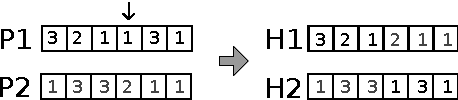
\includegraphics[scale=1]{img/fig2}
	\end{center}
	\label{fig:fig2}
	\caption{Explicación de violación de restricciones duras por cruzamiento}
\end{figure}

En la \textbf{Figura 2} de la sección~\ref{fig:fig2} podemos darnos cuenta que no estamos respetando las restricciones
duras de la cantidad de autos de Tipo 2 y 3, entonces si nos damos cuenta de que éste es un ejemplo
pequeño, la cantidad de restricciones violadas con una mayor cantidad de autos, será mucho mayor.

Como en el caso de los algoritmos evolutivos, el cruzamiento se encarga de explotar,
la explotación es suplida por la mutación \emph{Simulated Annealing}, ya que como bien sabemos,
a temperaturas altas, explora y a temperaturas bajas, explota.

\subsection{Elitismo}

Para la presente implementación, se consideró el elitismo como una pieza fundamental para poder
mejorar nuestra nuevas poblaciones.

Una vez que tengamos una población, el elitismo se encarga de buscar el individuo con más alto \emph{fitness},
y se reemplaza con el individuo que tenga el fitness más bajo, además siempre el mejor individuo de cada población
pasa directamente a la siguiente población, con lo cual se asegura no perder soluciones buenas con el pasar
de las poblaciones.

\subsection{Estructura del Algoritmo}

Tomando en cuenta toda la descripción anterior,
el algoritmo central sería:

\begin{verbatim}
	Inicio
	g <- 0 // numero de generaciones
	p <- 0 // numero de poblaciones
	Leer datos de entrada
    Población <- Generar población inicial
    Evaluar población

	    Mientras g < GENS
			Mientras n < POP - 1
				Selección individuo
				Mutación // Simulated Annealing + AM 
			Fin Mientras
			Elitismo
			Cambio de población // Población actual = Población nueva
			Evaluar población
	        n <- n + 1
	        p <- 0
		Fin Mientras
	Imprimir resultados
	Fin
\end{verbatim}

\subsection{Parámetros}

Para la presente implementación, se trabajó con una seria de constantes definidas antes de la ejecución del algoritmo,
las cuales fueron variadas para observar el desempeño del algoritmo, dejando las más apropiadas:
\begin{description}
	\item[VARS]: Número de variables (autos) de la secuencia, el cual es cambiado para cada experimento ($200$, $300$ y $400$).
	\item[POP]:  Tamaño de cada población.
	\item[GENS]: Número de generaciones.
	\item[PMUT]: Probabilidad de mutación. Se considero de que como no se realiza cruzamiento, la presente probabilidad se aumentó.
	\item[TMAX]: Temperatura Máxima para el \emph{Simulated Annealing}.
	\item[IMAX]: Número máximo de iteraciones para el \emph{Simulated Annealing}.
\end{description}


\section{Experimentos}
\label{sec:experimentos}
% Se necesita saber como experimentaron, como definieron par\'ametros,
%  como los fueron modificando, cuales problemas se trataron, instancias,
%  por que ocuparon esos problemas.

Los valores iniciales, eran menores a los señalados al final de la presente sección,
y para poder definirlo se fueron variando por separado.

Primero se fueron variando por separado los parámetros del \emph{algoritmo evolutivo},
donde se llegó a la conclusión, de que si la cantidad de las generaciones va aumentando,
y el tamaño de la población es muy grande, aparte de tardar demasiado en converger,
el desempeño no es bueno.

Luego se estableció la idea de tener poblaciones pequeñas, pero muchas generaciones,
así obtendremos mejores resultados, pero dependerá netamente, si las soluciones iniciales
son buenas, aquí el elitismo juega un papel sumamente importante.

En segundo lugar, las pruebas y modificaciones se realizaron con los parámetros de la
mutación \emph{simulated annealing}, donde se probaron distintos valores, que hicieron
llegar a la conclusión, de que es más apropiado, poseer un número no tan grande de iteraciones,
con respecto a la temperatura, pero la temperatura debe ser a lo más 1 orden de magnitud mayor
que el número de iteraciones.

De la misma forma, la temperatura, no debe tener valores muy elevados, porque no ayuda mucho
en encontrar mejores individuos, sobre todo en éste caso que era un \emph{simulated annealing}
con \emph{alguna mejora}.

Las instancias en las que se ejecutó el algoritmo, fueron los \emph{30 problemas difíciles} de
Caroline Gagne que se encuentran en el sitio de CSPLib~\cite{gagne}, por cada instancia se ejecutó
el presente algoritmo $100$ veces, para obtener una amplia gama de soluciones a distintas situaciones.

Los experimentos fueron realizados en un computador con las siguientes características:
\begin{itemize}
	\item Intel(R) Core(TM)2 Duo CPU 2.66\,[GHz]
	\item 4 Gigabyte RAM
	\item Sistema Operativo Fedora 12 para i686
\end{itemize}

Los parámetros utilizados en los experimentos, no fueron cambiados por cada población,
lo cual puede significar un desempeño inferior al sintonizarlos por en cada caso.

Los valores son:
\begin{itemize}
	\item VARS: 200, 300, 400 (dependiendo de cada caso)
	\item POP: 12
	\item GENS: 5000
	\item PMUT: 0.3
	\item TMAX: 100
	\item IMAX: 10
\end{itemize}


\section{Resultados}
\label{sec:resultados}
%El analisis de los datos obtenidos,
%	arrojara resultados que uds. deberan presentar en esta seccion.
%	Deben poner enfasis a los impactos del tema tecnologico en el
%	publico objetivo, y sus proyecciones.

En la sección anterior, pudimos darnos cuentas de los resultados de la encuesta realizada a personas que trabajan
en el mismo ambiente que se presenta en el trabajo, dándonos cuenta cuales herramientas utilizaban, si les eran útiles, etc,
pero ahora nos queremos enfocar en los \emph{impactos} principalmente, de nuestro tema principal, en el las personas estudiadas.

Con respecto a las tecnologías, podemos profundizar mucho acerca del proceso de \emph{selección}, \emph{desarrollo} y su propio \emph{uso},
y sobre todo, en el análisis a los impactos producidos por cada uno de los factores anteriormente señalados.
Éstos impactos, no influyen sólo en la persona, sino que van más allá, poseen una suerte de influencia en el quehacer humano y por ende
todo lo que lo rodea, \emph{alterando} su comportamiento.

Analizando uno de los investigadores más importantes en ésta área, McLuhan~\cite{mcluhan}, podemos obtener ciertas preguntas que nos van a servir para ver el impacto
de las tecnologías en nuestro ambiente.
Las preguntas son:
\begin{itemize}
	\item ¿Qué genera, crea o posibilita?
	\item ¿Qué preserva o aumenta?
 	\item ¿Qué recupera o revaloriza?
	\item ¿Qué reemplaza o deja obsoleto?
\end{itemize}

Las cuales debemos resolver por cada tecnología que se quiera evaluar.

Si consideramos las \emph{tecnologías de la información} como un elemento tecnológico, podemos pasar a responder dichas preguntas para el trabajo en general:
\begin{itemize}
	\item \emph{¿Qué genera, crea o posibilita?}\\
		Gracias a las tecnologías de la información, estamos generando nuevos caminos de comunicación para realizar determinadas actividades en cualquier área,
		creando así las instancias necesarias, para que la comunicación sea bastante directa, en comparación a metodologías antiguas.
		
		Tomando en cuenta lo anterior estamos posibilitando, que dos o más personas en lugares totalmente distintos en el mundo, puedan trabajar en conjunto,
		sin tener la necesidad de una cercanía física, lo cual nos sirve para obtener una especie de comodidad a la hora de trabajar.
		
	\item \emph{¿Qué preserva o aumenta?}\\
		Estamos preservando y aumentando en algunos casos, la cantidad de trabajo realizado en conjunto, pues tenemos que tener en cuenta que al existir una
		comunicación más fluida, aumentamos la relación de dos distintas organizaciones, en un proyecto determinado.

		Por otra parte, aumenta la capacidad de que grupos pequeños de estudiantes con una misma motivación, puedan realizar actividades que contribuyan
		a proyectos mundiales, en los cuales por una razón económica, o quizás considerando la comodidad, no pueden estar presentes en un determinado lugar
		en el mundo.
	
		Tomando en cuenta ambos puntos, podemos darnos cuenta, que el crecimiento como profesional de un determinado estudiante, crece enormemente,
		pues ya no está sometido a un estilo de trabajo local, de su universidad y/o entorno, conociendo nuevas costumbres, estilos de trabajo, etc.

 	\item \emph{¿Qué recupera o revaloriza?}\\
		Al momento de abastecernos con todas los recursos necesarios utilizando tecnologías de la información, podemos comenzar a recuperar valores o 
		buenas costumbres al momento de realizar un proyecto, revalorizando el trabajo realizado; con ésto nos referimos a que cuando uno se encuentra
		en un establecimiento educacional y realiza cierto proyecto, no tiene el mismo valor, obtener una buena calificación en una asignatura determinada,
		que se reconozca el mismo trabajo, por una organización mundialmente conocida.

		Comenzamos a darnos cuenta, que junto a la perseverancia podemos llegar a cumplir objetivos bastante ambiciosos.		

	\item \emph{¿Qué reemplaza o deja obsoleto?}\\
		Si el uso de la tecnología no es utilizado de una buena forma, es decir, no abusando y llevando al máximo las comodidades que nos ofrece,
		se puede transformar en algo negativo para una persona o un entorno social, reemplazando todo lo que son las relaciones interpersonales,
		el poder entablar una conversación ``en persona'' con algún otro individuo.

		Por otro lado, la tecnología actual ha dejado de lado (no del todo) a medios de comunicación antiguos, como lo son las cartas tradicionales,
		el Fax, el telégrafo, etc , que en su tiempo, fueron lo último de la tecnología, con lo que podemos decir, que la misma tecnología,
		deja obsoleta a la tecnología.

\end{itemize}

Considerando que éste análisis puedo no ser del todo completo con respecto a la apreciación de los impactos de las \emph{tecnologías de la información},
existen trabajos complementarios para comprender mucho mejor los fenómenos observados.

Para identificar mejor los impactos, ya sean negativos o positivos de las distintas actividades relacionadas con tecnologías sobre las personas,
Solivérez~\cite{soliverez} propone un nuevo conjunto de preguntas:
\begin{itemize}
	\item \emph{Impacto práctico:}
	\begin{itemize}
		\item ¿Para qué sirve?
		\item ¿Qué permite hacer que sin ella sería imposible?
		\item ¿Qué facilita?
	\end{itemize}
	\item \emph{Impacto simbólico:}
	\begin{itemize}
		\item ¿Qué simboliza o representa?
		\item ¿Qué connota?
	\end{itemize}
	\item \emph{Impacto tecnológico:}
	\begin{itemize}
		\item ¿Qué objetos o saberes técnicos preexistentes lo hacen posible?
		\item ¿Qué reemplaza o deja obsoleto?
		\item ¿Qué disminuye o hace menos probable?
		\item ¿Qué recupera o revaloriza?
		\item ¿Qué obstáculos al desarrollo de otras tecnologías elimina?
	\end{itemize}
	\item \emph{Impacto ambiental:}
	\begin{itemize}
		\item ¿El uso de qué recursos aumenta, disminuye o reemplaza?
		\item ¿Qué residuos o emanaciones produce?
		\item ¿Qué efectos tiene sobre la vida animal y vegetal?
	\end{itemize}
	\item \emph{Impacto ético:}
	\begin{itemize}
		\item ¿Qué necesidad humana básica permite satisfacer mejor?
		\item ¿Qué deseos genera o potencia?
		\item ¿Qué daños reversibles o irreversibles causa?
		\item ¿Qué alternativas más beneficiosas existen?
	\end{itemize}
	\item \emph{Impacto epistemológico:}
	\begin{itemize}
		\item ¿Qué conocimientos previos cuestiona?
		\item ¿Qué nuevos campos de conocimiento abre o potencia?
	\end{itemize}
\end{itemize}

Las cuales nos van a permitir obtener un argumento mas completo a la hora de analizar los impactos que nos interesan.
Para éste caso sólo nos limitaremos a analizar el \emph{Impacto Ético}.

\begin{itemize}
	\item \emph{¿Qué necesidad humana básica permite satisfacer mejor?}\\
		La necesidad de la comunicación con personas que no se encuentres cerca, geográficamente hablando.
		Estamos mucho más conectados con todo el mundo, por lo que no importa el lugar, siempre podremos
		estar en contacto de las personas que necesitemos.

	\item \emph{¿Qué deseos genera o potencia?}\\
		Los deseos de continuar con distintos proyectos, en nuevas organizaciones, generar grupos de trabajo,
		potenciando el trabajo en equipo internacional, lo cual se ve beneficiado al momento de querer
		generar lazos aún más fuertes, donde se recurren a eventos como \emph{Workshops} en algún lugar del mundo,
		donde aparte de conocer a las personas e interactuar con ellas, se crean nuevos lazos que podrán estar
		vigentes con el pasar del tiempo, gracias a la tecnología de la información.

	\item \emph{¿Qué daños reversibles o irreversibles causa?}\\
		Con respecto a los daños reversibles, tenemos la adicción a la información que se ha dado en varias personas,
		tomando las palabras del último trabajo del ramo, puede producirse una esclavitud tecnológica.
		Por otro lado tenemos el problema anteriormente señalado, que es la pérdida de las relaciones sociales,
		que puede ser controlada, moderando el uso de los medios de comunicación tecnológicos actuales.

		Ahora considerando los daños irreversibles, tenemos que la actitud de algunas personas puede transformarse
		negativamente a asumir la facilidad de obtener o realizar tareas, sin ir más lejos los daños al lenguaje,
		que hoy en día la juventud posee, que tienen como fin sólo agilizar la comunicación, alterando el mensaje.
		
		Pero concentrándonos en nuestro problema, el único problema que se puede temer,
		son la pérdida de las relaciones interpersonales, que si bien es cierto considerando las colaboraciones
		internacionales es positivo que la gente trabaje, no hay que producir cierta esclavitud, no podemos vivir
		sin relacionarnos con otras personas, ya que eso es lo que sustenta la sociedad.

	\item \emph{¿Qué alternativas más beneficiosas existen?}\\
		Más que buscar una alternativa a las tecnologías de la información, tenemos el fiel pensamiento de que
		no hay que buscar alternativas sino que hay que aprender a vivir con la tecnología, que hoy por hoy,
		nadie sabe utilizar de la mejor forma la tecnología.

		¿Tenemos clara la noción de lo bueno y lo malo? a veces la información puede alterar nuestra percepción
		de ciertas actividades, pero en el caso de las relaciones internacionales, no se ve tanta coherencia
		a la presente idea.
\end{itemize}


\section{Conclusiones}
\label{sec:conclusiones}
%De acuerdo a la introducci\'on que se hizo, entregar afirmaciones
%  basadas en los experimientos y sus resultados.

A primera vista, los resultados obtenidos en la presente implementación, superan en gran medida a los óptimos encontrados
en todos estos años, donde distintas personas, han utilizado, variadas técnicas para poder resolver el \emph{Car Sequencing Problem}
de la mejor manera, considerando así, que se pudieron haber utilizado técnicas completas, que si bien es cierto, pueden demorar mucho,
van a encontrar el \emph{óptimo global} de un determinado problema, lo cual se diferencia notoriamente con las técnicas incompletas,
como es el caso de ka presente implementación, donde sólo se puede encontrar un \emph{óptimo local}.

Al mirar el gráfico podemos darnos cuenta, de que la distribución de la cantidad de restricciones violadas, poseen un comportamiento
bastante similar, guardando las proporciones de la cantidad de violaciones, lo que nos hace deducir, de que sólo nos falta un poco
más de control y sintonización de los parámetros utilizados, para acercarnos aún más a soluciones más óptimas.

Siguiendo con el análisis de los experimentos, podemos darnos cuenta de que si bien es cierto, las soluciones violan una cantidad
considerable de restricciones, estamos sacrificando una buena solución, por un corto tiempo de ejecución, el cual en algunos casos,
sólo llega a durar 1 minuto, lo que comparado con el tiempo de alguna técnica completa, que puede durar días, nos beneficia de cierta manera.

Con respecto a la representación del problema, existen ciertos pros y contras.
Primero que todo la representación que se utilizó en la presente implementación,
consiste en una del tipo no-binaría, por lo que no es tan fácil utilizar los típicos movimientos de las representaciones binarias,
como lo son el \emph{bit-flip} y el \emph{cruzamiento en un punto}, ya que estaríamos violando las restricciones duras del problema,
por lo cual en la presente implementación, por ejemplo, no se utilizó un operador de cruzamiento y sólo se deposito la confianza,
en la mutación con \emph{Simulated Annealing} que se encargó tanto de explorar como de explotar.

Según lo anteriormente dicho, el no poseer un operador de cruzamiento, puede haber perjudicado la explotación del presente algoritmo
evolutivo, y por ende, entorpecido la búsqueda de un óptimo local. Aunque los resultados no fueron del todo malos, por lo que el simulated annealing
hizo su trabajo explorando y explotando, pero no de la forma más apropiada.

Otro punto importante en la presente implementación, es la forma en la cual se genera la población inicial.
Como ya hemos mencionado anteriormente, lo favorable del método utilizado es que se generan soluciones factibles,
es decir, que cumplen las restricciones duras, pero por otro lado, éstas se generan de forma aleatoria, lo cual indica,
que quizás utilizando alguna técnica de construcción de individuos más apropiada, como Greedy o GRASP, la calidad de la
población inicial aumentaría, lo cual sería interesante como trabajo futuro.


Con respecto a la mutación con simulated annealing, cabe señalar que existen algunos aspectos que pueden ser mejorados,
como por ejemplo un control de la temperatura, pues en la presente implementación, la temperatura disminuye cada 3 iteraciones,
lo que si tomamos en cuenta un control más riguroso, como comparar la calidad de las soluciones generadas, podríamos
realizar los cambios en la temperatura, a medida que el algoritmo se comporta de una forma más apropiada.


Finalmente, es posible mejorar la presente implementación de un algoritmo evolutivo aumentando la exploración,
que en éste caso significa poder mejorar lo que es la mutación, ya que dentro del simulated annealing, el movimiento
no es muy apropiado, y quizás el sólo hecho de mejorar el movimiento de la mutación simulated annealing, puede
traer un mejor desempeño en nuestro algoritmo. Otra forma podría ser cambiar el método de la ruleta, pues si bien es cierto,
le entrega una mayor probabilidad para escoger los mejores individuos, no nos prohibe elegir malos individuos, lo que
perjudica a nuestra siguiente población, y por ende a la solución del problema.


% OLD

%Conclusiones revelantes del estudio realizado.

%En el presente informe se ha dado un estado del arte de un problema muy popular
%en el área de la inteligencia artificial, el \emph{Car Sequencing Problem}, siendo éste
%una variación de otro problema connotado llamado \emph{Job Shop Scheduling}.
%Es tanto la importancia del presente problema, que la \emph{French Society of Operations
%Research and Decision-Making Aid} ha decidido ya hace varios años, comenzar lo que se denomina
%\emph{The ROADEF challenge} cada dos años, teniendo como objetivo central,  permitir a las personas
%que se desarrollan en el área de la industria el presenciar todos los avances y evoluciones
%en el ámbito de la Investigación de Operaciones y Análisis de Decisiones, pero no sólo eso
%sino el poder enfrentar directamente problemas decisionales complejos, que ocurren en la industria.
%Siguiendo la idea anterior, lo importante de éste \emph{Challenge} es que en el 2005, se consideró
%como tema principal el \emph{Car Sequencing Problem} debido a la propuesta que realizó RENAULT,
%por lo cual uno podrá imaginar la cantidad de avances que se produjeron, pues cada participante
%abordaba el problema desde una metodología distinta.
%
%Por otra parte, pareciera que un problema relacionado a \emph{ordenar} un conjunto de vehículos
%para ser ensamblados y así obtener el orden más óptimo, no es una tarea difícil, pero claramente
%debido a la complejidad que otorgan las restricciones y de que es un problema de la vida real,
%presenta un grado de dificultad mayor, lo cual queda reflejado por la cantidad de publicaciones 
%e investigaciones que hay al respecto.
%
%Se dieron a conocer también, tres áreas para atacar el presente problema.
%Por un lado tenemos los métodos heurísticos que como bien sabemos, es prácticamente jugar a la ruleta
%rusa con nuestra investigación, pues la heurística solamente selecciona un objetivo de los dos provenientes
%de la definición, una buena solución o un buen tiempo de ejecución. Pero también se presenta que la heurística
%es un mecanismo confiable para decidir \emph{utilizarlo} como un apoyo, mas que utilizarlo solo.
%
%Siguiendo con los mecanismos planteados, se vieron también los  métodos exactos,
%es decir, técnicas de optimización, donde podemos encontrar la \emph{programación lineal entera},
%\emph{branch and bound} y \emph{local search}, los cuales se dedicaban netamente a construir una
%solución óptima a partir de los datos que el mismo problema nos entrega. El único problema que tienen
%éstas técnicas es que la complejidad temporal va a crecer demasiado con respecto al tamaño de nuestro
%\emph{input} del algoritmo.
%
%Dentro de toda la lectura realizada para las distintas técnicas, pude percatarme que las mejores soluciones
%siempre son variaciones de métodos o tomar dos técnicas como complementarias, por ejemplo uno de los
%mejores resultados fue la combinación de un \emph{Ant Colony Optimization} con una heurística dinámica,
%pues claramente se nos señala que el buen uso de una heurística es crucial, es decir, hay que preocuparse
%de leer los estudios que se han publicado, par ver cual es la combinación más óptima.
%
%Finalmente, es impresionante la cantidad de estudios con respecto a éste problema en particular,
%por lo que podemos darnos cuenta que muchos centros de investigación han dedicado tiempo valioso
%para la resolución óptima del \emph{Car Sequencing Problem}, pero no tanto la versión que se estudió,
%que es la propuesta por Parello~\cite{parello}, sino mas bien al desafío de la ROADEF.


%%%

\section{Bibliografía}
\bibliography{informe2}

\end{document} 
